\section{Programs}
We decided to focus on a single problem domain and test different implementations for the same problem, we decide to use pathfinder algorithms as the domain problem.\newline

\noindent
We chose these three algorithms:
\begin{enumerate}
    \item A*
    \item Dijkstra algorithm
    \item Yen's algorithm
\end{enumerate}

\pagebreak

\subsection{A*}

Code implementation: \newline
\url{https://gist.github.com/Nicholas-Swift/003e1932ef2804bebef2710527008f44} \newline\newline

\noindent
In the A* program we see that the most difficult part of the program is from line \textbf{79-97} because there are three nested loops with multiple conditionals.
\begin{center}
    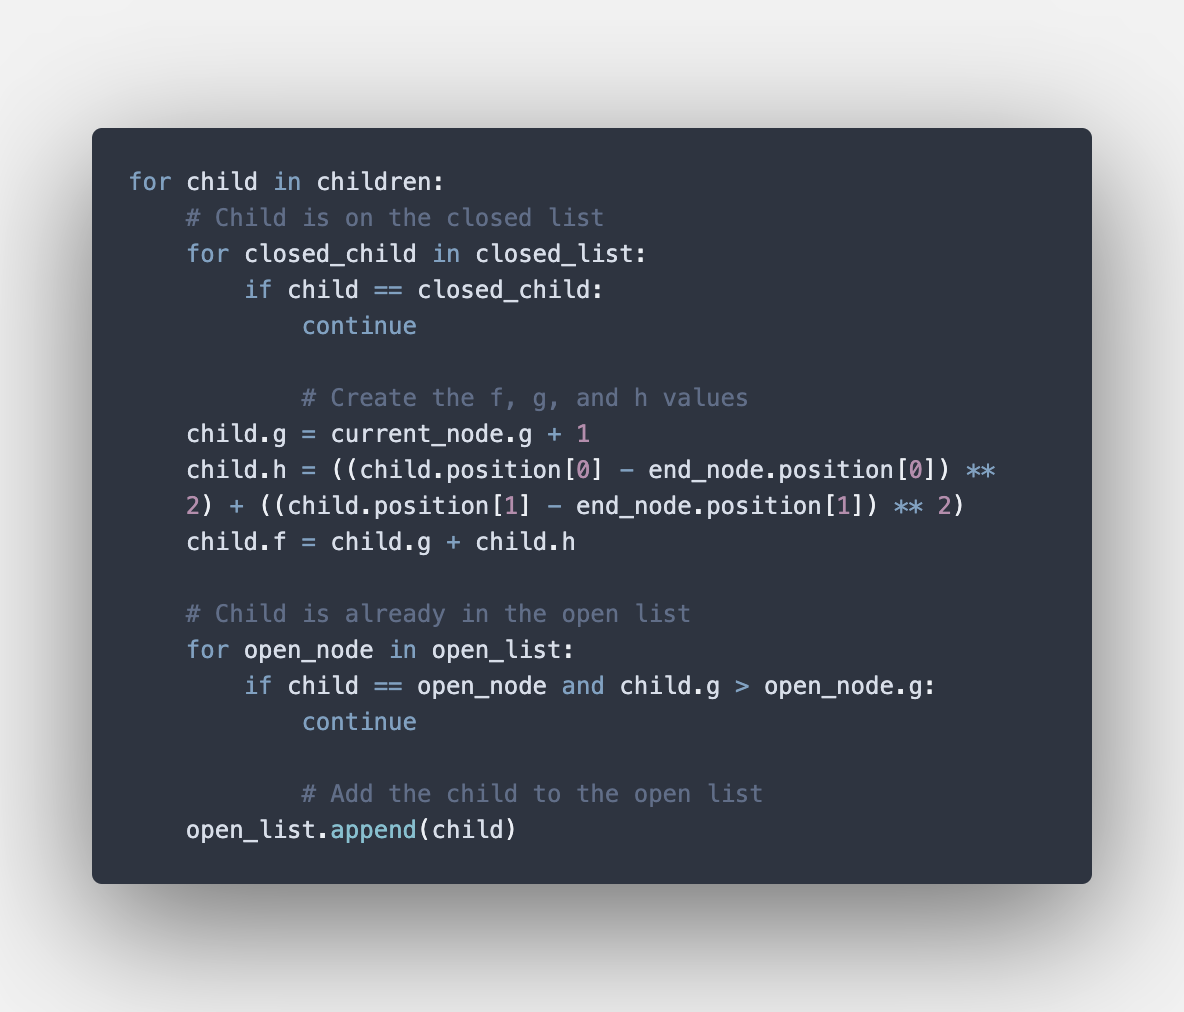
\includegraphics[scale=0.3]{a_star.png}    
\end{center}

\pagebreak

\subsection{Dijkstra algorithm}
Code implementation: \newline
\url{https://gist.github.com/econchick/4666413} \newline\newline

\noindent
For Dijkstra, we see that the most complex section of the code is from line \textbf{22-41} because there are two for loops with nested conditionals.

\begin{center}
    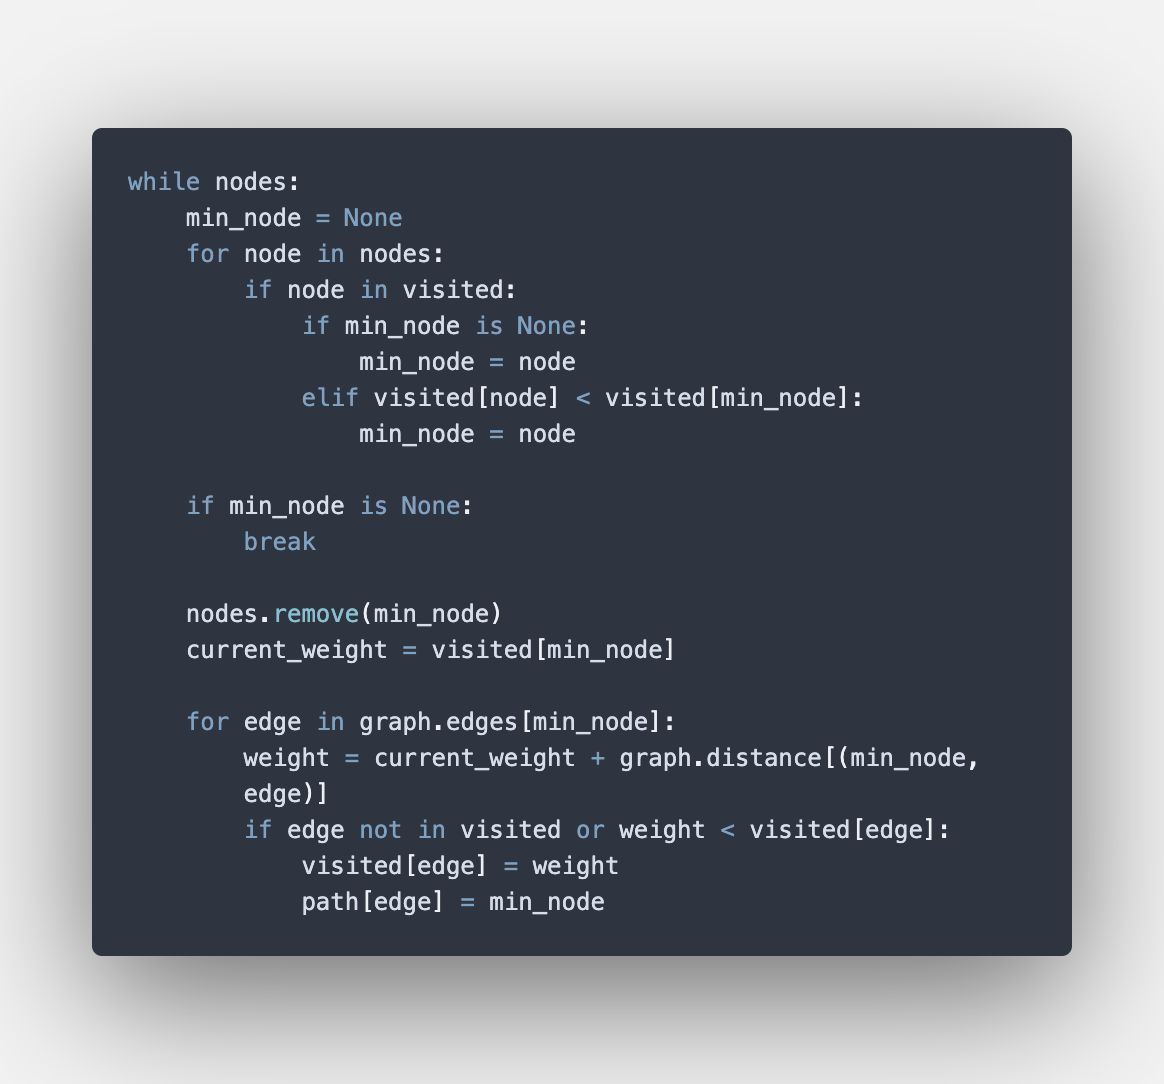
\includegraphics[scale=0.3]{dijkstra.png}    
\end{center}

\pagebreak

\subsection{Yen's algorithm}
Code implementation: \newline
\url{https://gist.github.com/ALenfant/5491853} \newline\newline

\noindent
In Yen's algorithm, the most complex sections are from line \textbf{23-38} because we have 3 nested loops with nested conditionals (\textbf{35-38}).

\begin{center}
    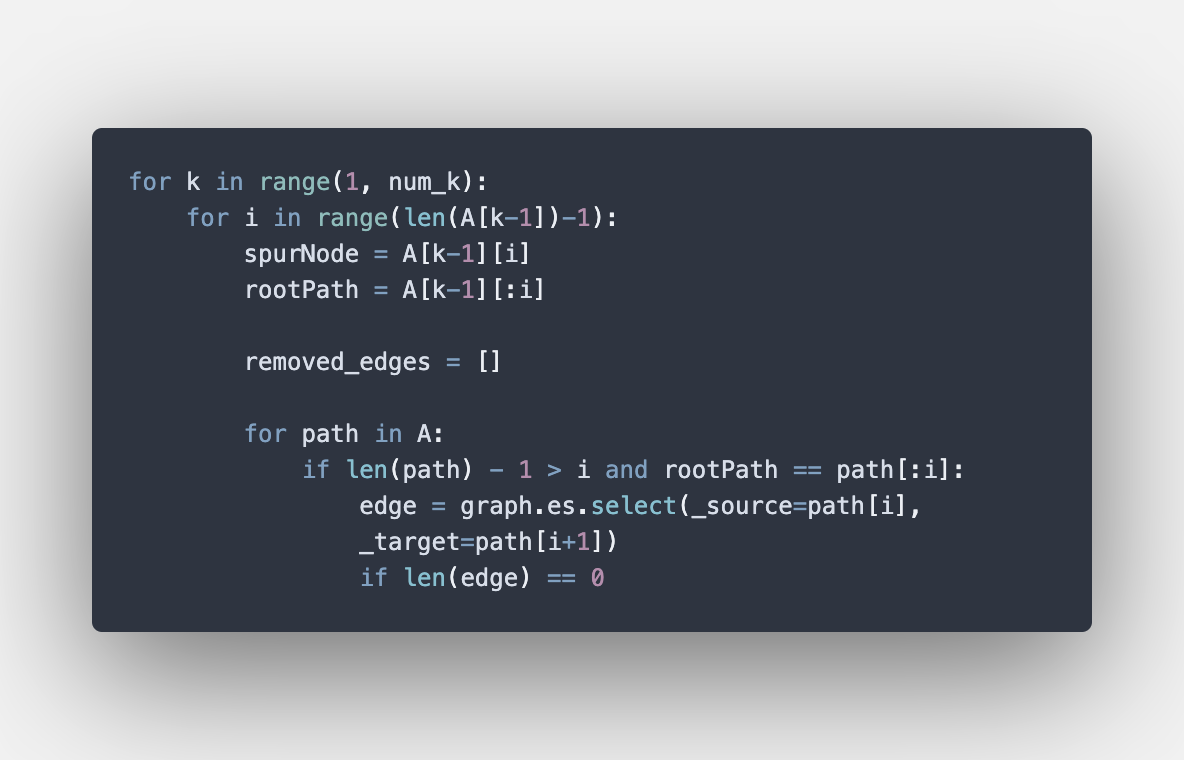
\includegraphics[scale=0.3]{yen.png}    
\end{center}

\subsection{Preliminary Conclusions}
We think that difficulty is:
\begin{enumerate}
    \item Yen's algorithm
    \item A*
    \item Dijkstra algorithm
\end{enumerate}

Yen's algorithm is the most complex one, A* the second and Dijkstra the least complex. The reason behind this is because Yen's algorithm has 3 nested for loops and also a while loops, Dijkstra being the easiest because it has less LOC and there are no nested for-loops, leaving the A* in the second most complex.

\pagebreak

\section{Tool Analysis}

We use \textbf{radon} to get the CC, MI, and Halstead metrics. \newline\newline
\url{https://radon.readthedocs.io/en/latest/}

\begin{center}
    \begin{tabular}{|p{3cm} | p{2cm} | p{2cm}| p{2cm}|}
        \hline
        \textbf{Metric} & \textbf{A*} & \textbf{Yen} & \textbf{Dijkstra}\\
        \hline
        CC & 18 & 11 & 3\\ 
        \hline
        MI & 64.73 & 72.97 & 61.10 \\  
        \hline
        h1 & 11 & 7 & 6 \\
        \hline
        h2 & 45 & 23 & 13  \\
        \hline
        N1 & 35 & 19 & 8  \\
        \hline
        N2 & 65 & 38 & 16 \\
        \hline
        Vocabulary & 56 & 30 & 19  \\
        \hline
        Length & 100 & 57 & 24  \\
        \hline
        Calculated Length & 285.19 & 123.69 & 63.61 \\
        \hline
        Volume & 580.74 & 279.69 & 101.95  \\
        \hline
        Difficulty & 7.94 & 5.78 & 3.69 \\
        \hline
        Effort & 4613.62 & 1617.35 & 376.43 \\
        \hline
        Time & 256.31 & 89.85 & 20.91 \\
        \hline
        Bugs & 0.19 & 0.093 &  0.03\\
        \hline
    \end{tabular}
\end{center}

\noindent
By looking at the metrics we can see that A* is the most complex one, not only because of the CC but also with some of the Halstead metrics, the program itself is longer, the volume is way bigger, double of Yen algorithm and 5 times the size of Dijkstra. A* also is more difficult than the other two algorithms and takes more effort.

\pagebreak

\section{Comparison}
\subsection{How does the tool results compare to your intuition?}
Our intuition matches the one from the tool at least in the fact that the least complex is the Dijkstra algorithm, but we miss the fact that the A* was more complex than Yen's algorithm, could be the fact that A* has more readable variables and a better line of sight, \textit{fewer indentation levels}, than Yen's, perhaps if the yen's implementation had better naming conventions our intuition would say something different.

\subsection{Are they consistent?}
Only with the fact that the Dijkstra algorithm is the least complex one of the three.
\subsection{What did you think of the code analysis tool?}
Is easy to use and you are able to get a lot of metrics from the program, while also generate a nice output if required.

\subsection{Good or not so Good? Why?}
I'ts really good because:
\begin{enumerate}
    \item Is easy to install
    \item It has a helper function in the tool itself
    \item Has output controls
    \item Provides different types of metrics
    \item It's open-source
\end{enumerate}

\pagebreak

\section{Viewpoints}
From the following viewpoints:
\begin{enumerate}
    \item LOC is adequate as an indicator of software complexity
    \item CC is more useful than LOC in measuring software complexity
\end{enumerate}

\noindent 
We said that CC is more useful than LOC to measure software complexity because you can increase the LOC to improve readability, or you group some behavior in a function, and the function declaration itself will increase the lines a little bit but could be reused in the future, while the CC contains the logic of the application itself, it doesn't matter if the code is right there or in another function the loops and the conditional statements are the ones that control that value.